% 2017 全国Ⅰ卷 文6：选项 (C)(D) 的两个正方体
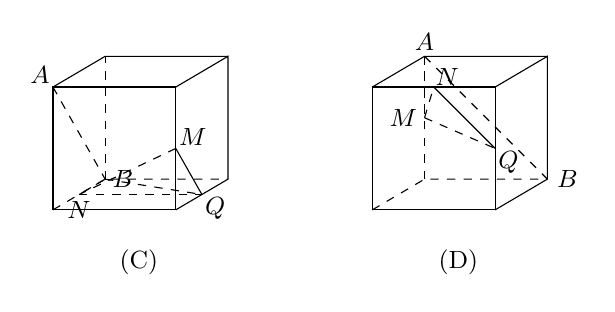
\begin{tikzpicture}[scale=0.78, font=\small]
  % ---------- (C)：A 前左上，B 后左下；M 前右竖棱中点，N 底面左棱中点，Q 底面右棱中点 ----------
  \begin{scope}
    \draw (0,0) rectangle (2,2);
    \draw (2,0) -- (2.85,0.5) -- (2.85,2.5) -- (2,2);
    \draw (0,2) -- (0.85,2.5) -- (2.85,2.5);
    \draw[dashed] (0,0) -- (0.85,0.5) -- (2.85,0.5);
    \draw[dashed] (0.85,0.5) -- (0.85,2.5);
    \coordinate (A) at (0,2);
    \coordinate (B) at (0.85,0.5);
    \coordinate (M) at (2,1);
    \coordinate (N) at (0.425,0.25);
    \coordinate (Q) at (2.425,0.25);
    \draw[dashed] (A) -- (B);
    \draw[dashed] (B) -- (N) (B) -- (Q);   % 到 M N Q 的示意连线在底面/内部
    \draw[dashed] (N) -- (Q);
    \draw (M) -- (Q);
    \draw[dashed] (M) -- (N);
    \node[above left, inner sep=1pt] at (A) {$A$};
    \node[right, inner sep=2.5pt] at (B) {$B$};
    \node[above right, inner sep=1pt] at (M) {$M$};
    \node[below, inner sep=2.5pt] at (N) {$N$};
    \node[below right, inner sep=1pt] at (Q) {$Q$};
    \node at (1.4,-0.85) {(C)};
  \end{scope}
  % ---------- (D)：A 后左上，B 后右下；M 后左竖棱中点，N 前上棱中点，Q 前右竖棱中点 ----------
  \begin{scope}[xshift=5.2cm]
    \draw (0,0) rectangle (2,2);
    \draw (2,0) -- (2.85,0.5) -- (2.85,2.5) -- (2,2);
    \draw (0,2) -- (0.85,2.5) -- (2.85,2.5);
    \draw[dashed] (0,0) -- (0.85,0.5) -- (2.85,0.5);
    \draw[dashed] (0.85,0.5) -- (0.85,2.5);
    \coordinate (A) at (0.85,2.5);
    \coordinate (B) at (2.85,0.5);
    \coordinate (M) at (0.85,1.5);
    \coordinate (N) at (1,2);
    \coordinate (Q) at (2,1);
    \draw[dashed] (A) -- (B);
    \draw[dashed] (A) -- (M);            % A 沿后左竖棱到 M 已被棱覆盖，此线与棱重合
    \draw (N) -- (Q);
    \draw[dashed] (M) -- (N) (M) -- (Q);
    \node[above, inner sep=2pt] at (A) {$A$};
    \node[right] at (B) {$B$};
    \node[left, inner sep=2.5pt] at (M) {$M$};
    \node[above right, inner sep=0.5pt] at (N) {$N$};
    \node[below right, inner sep=1pt] at (Q) {$Q$};
    \node at (1.4,-0.85) {(D)};
  \end{scope}
\end{tikzpicture}
